\chapter{Evaluation of \glsentrytext{bosss} for Viscid Flows}
\label{viscousCylinder}
In this chapter, we aim at validating \gls{bosss} for viscid flows with \gls{ibm}s. In order to have a good comparable result, we will once again regard the flow around a cylinder as in chapter \cref{eulerVerification}. 
The viscous flow around a cylinder has been approached by many papers both experimentally and numerically, e.g. \textcite{williamson1996vortex}, \textcite{FLM:14223}, \textcite{canutoTaira}, though very few numerical approaches use a \gls{rkdg} method combined with immersed boundaries. In order to validate the \gls{bosss} code with immersed boundaries not only for the Euler equations as we did in chapter \cref{eulerVerification} but also for the viscous case we will now consider different Reynolds numbers for the steady and unsteady flow and compare our results to those of other studies.

\section{Theory}
	The flow around a viscous cylinder can be divided into different sections depending on the Reynolds number as shown in \cref{fig:overview}. The first section applies for Reynolds numbers $0 < \text{Re} < 40-50$ characterised by a laminar steady flow. In that regime, a recirculation region with two symmetric vortices with opposite directions is comprised by the wake. The flow can be described using the wake separation length $W^*$.\\\\
	\begin{figure}[htp]
		\centering
		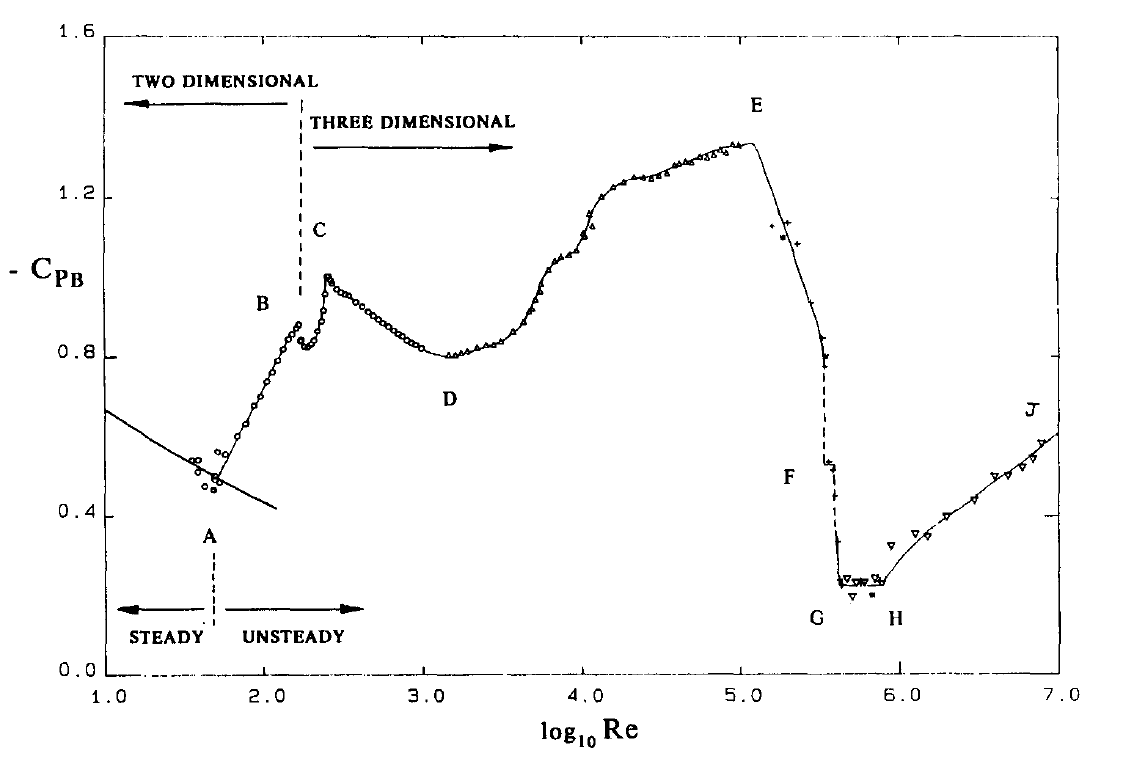
\includegraphics[height=8cm]{overviewCylinderReynolds_Williamson.PNG}
		\caption{Overview of Base Suction Coefficients over Reynolds Number \cite{williamson1996vortex}}
		\label{fig:overview}
	\end{figure} 
	The second section contains all other Reynolds number $\text{Re}> 40-50$ and thus describes the unsteady flow. It can be subdivided in several subsections \cite{williamson1996vortex}:
	\begin{itemize}
		\item $40-50 < \text{Re} < 190$: laminar vortex shedding,
		\item $190 < \text{Re} < 260$: \gls{3d} wake-transition regime,
		\item $260 < \text{Re} < 1000$: increasing disorder in the fine-scale three-dimensionalities,
		\item $1000 < \text{Re} < 200000$: shear layer transition regime,
		\item $200000 < \text{Re}$: critical transition, supercritical regime and post-critical regime.
	\end{itemize}
	
	As we will only discuss Reynolds numbers up to $\text{Re} = 200$, the important phases for us are the laminar steady regime and the laminar vortex shedding. At around $\text{Re} = 190$, the three dimensionality of the system has an incrementing influence on the flow; for we only analyse the \gls{2d} model of the experiment we stop at $\text{Re} = 200$ expecting slight deflection in our results.
	
	\subsection{The Laminar Steady Regime}
	
	At Reynolds numbers below 50, the flow forms a steady recirculation region, characterised by the wake separation length  $W^*$. It is built by two symmetrically placed vortices on each side of the wake as can be seen in \cref{fig:steady}. It has been shown experimentally as well as numerically that the wake separation length increases with increasing Reynolds number. 
		\begin{figure}[htp]
			\centering
			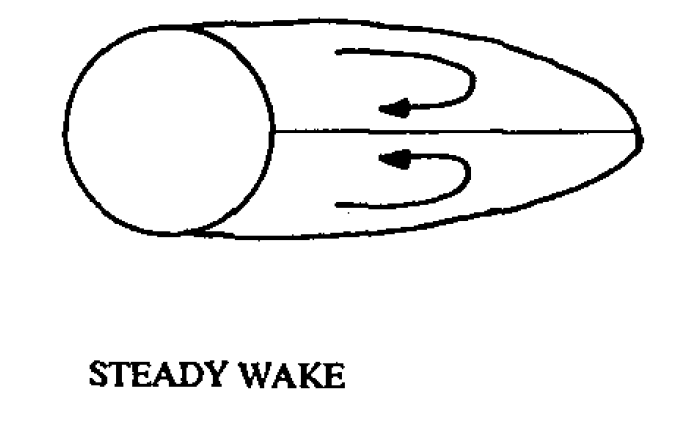
\includegraphics[height=4cm]{steadyFlow_Williamson.PNG}
			\caption{Recirculation Region \cite{williamson1996vortex}}
			\label{fig:steady}
		\end{figure}
	\subsection{Laminar Vortex Shedding}
	For Reynolds numbers of between 50 and 200 the recirculation region develops instabilities leading to the development of turbulence in the wake. This results into fully periodic vortex shedding, known as the Kármán vortex street, as can be seen in \cref{fig:unsteady}. With increasing Reynolds number the amplitudes of the drag and lift coefficients increase while the Strouhal number and frequency, respectively, decrease.
	
		\begin{figure}[htp]
			\centering
			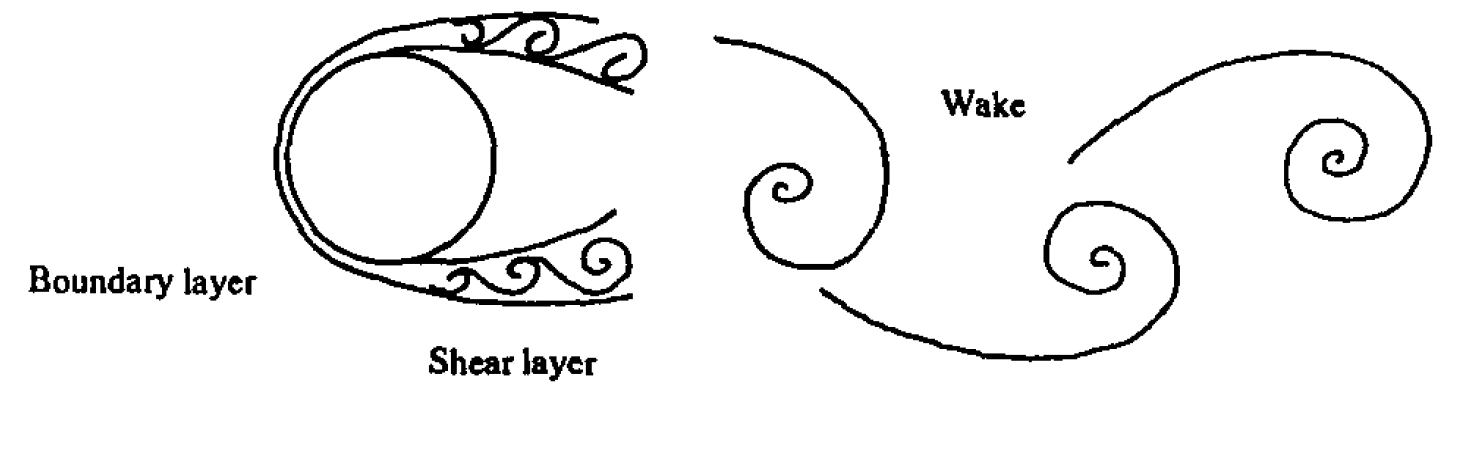
\includegraphics[height=4cm]{unsteady_Williamson.PNG}
			\caption{Kármán Vortex Street \cite{williamson1996vortex}}
			\label{fig:unsteady}
		\end{figure}
		
\section{Simulations}
	In this section we will compare the lift and drag coefficients $C_L$ and $C_D$ at different Reynolds numbers and mesh sizes at a constant agglomeration threshold of $0.3$, different polynomial degrees of 1, 2 and 3 and meshes of $40 \times 40$, $60 \times 60$ and $80 \times 80$ cells. The meshes can be found in the appendix. \\\indent
	The different simulation properties will be abbreviated as DG $+$ \textit{polynomial degree} $+$ CpD $+$ \textit{number of cells per direction}, e.g. DG2CpD80 for a simulation with polynomial degree 2 and $80 \times 80$ cells.\\
	In \cref{DOF} you can see the total \gls{dof} for each simulation taking into account the \gls{dof}s produced by order 1, 2 and 3 with 3, 6 and 10 \gls{dof}s per cell.
	
	\begin{table}[htp]
		\centering
		\def\arraystretch{1.5}
			\begin{tabular}{|c|c|c|c|c|}
				\hline
				\multicolumn{2}{|c|}{\multirow{2}{*}{DoF}} & \multicolumn{3}{c|}{CpD} \\ \cline{3-5} 
				\multicolumn{2}{|c|}{}                       & 40     & 60    & 80    \\ \hline
				\multirow{3}{*}{DG}            & 1           &    4800    &    10800   &    19200    \\ \cline{2-5} 
				& 2           &    9600    &   21600    &    38400    \\ \cline{2-5} 
				& 3           &      16000  &   36000    &   64000     \\ \hline
			\end{tabular}
			\caption{Degrees of Freedom for Different Simulation Properties}	
			\label{DOF}
	\end{table}
	
	 The drag and lift coefficients are defined as
	\begin{align}
		C_D = \dfrac{d}{q_\infty L_\infty} \\
		C_L = \dfrac{l}{q_\infty L_\infty}
	\end{align}
	with the dynamic pressure $q_\infty = \dfrac{1}{2} \rho_\infty V_\infty^2$. For we set $L_\infty = \rho_\infty = V_\infty = 1$ in our boundary and initial conditions, we can assume
	\begin{align}
		C_D = 2 \cdot d \\
		C_L = 2 \cdot l,
	\end{align}
	with the drag and lift forces $d$ and $l$ provided from the calculation. \\\\
	As we expect asymmetrical oscillations of the flow with higher Reynolds numbers, we cannot limit the domain to the upper or lower half as we did in \cref{eulerVerification}. In order to reduce the runtime of the calculations, we will compute a smaller domain with $-20 \leq x \leq 20$, $-20 \leq y \leq 20$ and the cylinder radius $r = 0.5$ during the simulations.
	We will use a rectilinear mesh that is finer near the cylinder with the level set $\varphi = x^2 + y^2 -0.5^2$, an isothermal wall boundary condition at the cylinder wall and supersonic inlet boundary conditions for the domain borders that shall prevent the reflection of the initial wave.  \\\\
		
	\subsection{Steady State Simulations ($\text{Re} < 40-50$)}
	For the steady state simulations, we can use the wake separation length $W^*$ as an additional variable to compare to other simulations.
			\begin{figure}[htp]
				\centering
				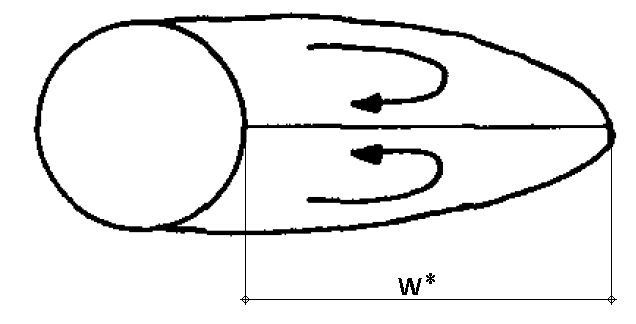
\includegraphics[height=4cm]{steadyFlow_modifiedWilliamson.PNG}
				\caption{Wake separation length, taken from \cite{williamson1996vortex}, modified }
				\label{fig:wakeSeparation}
			\end{figure} 
	It can be found from examining the x-velocity $U$ at $y=0$; the x-position where $U$ changes its sign should be the end position of the wake.

	\subsubsection{Simulation at Reynolds Number 20}
	We will now simulate the flow at $\text{Re}=20$ and compare our results to several experimental and numerical results as shown in \cref{tab:table20}. The results are divided into three categories: experimental, numerical incompressible and numerical compressible in order to coincide with the arrangement given by \textcite{ayers}.Furthermore the results are divided into \gls{2d} and \gls{3d} simulations which should not produce large differences as long as we are regarding low Reynolds numbers. The values that were produced by Brehm et al. [2015] using $\text{Ma} = 0.1$ as well as those that were simulated as incompressible flows can still be compared as in these low Mach numbers the compressibility does not have a great effect on the flow.

\begin{table}[htp]
	\centering
	\begin{tabular}{|l|l|c|c|c|}
		\hline
		\rule{0pt}{2,3ex}$\text{Re}=20$                              & Source                             & \gls{2d}/\gls{3d} & $W^*$ & $C_D$ \\ \hline
		\rule{0pt}{2,3ex}\multirow{3}{*}{\begin{minipage}{2.8cm}Numerical --\newline Incompressible\end{minipage}} & Dennis et al {[}1970{]}            & \gls{2d}    & $0.94$     & $2.05$     \\ \cline{2-5} 
		\rule{0pt}{2,3ex}& Forberg {[}1980{]}                 & \gls{2d}    & $0.91$     & $2.00$     \\ \cline{2-5} 
		\rule{0pt}{2,3ex}& Linnick et al. {[}2005{]}          & \gls{2d}    &$ 0.93 $    & $2.06$     \\ \hline
		\rule{0pt}{2,3ex}\multirow{2}{*}{Experimental}               & Coutanceau et al. {[}1978{]}       & -     & 0.93    & -     \\ \cline{2-5} 
		\rule{0pt}{2,3ex}& Tritton {[}1959{]}                 & -     & -     & $2.09$     \\ \hline
		\rule{0pt}{2,3ex}\multirow{3}{*}{\begin{minipage}{2.8cm}Numerical --\newline Compressible\end{minipage}}     & Brehm et al. {[}2015{]} (Ma = 0.1) & \gls{3d}    & $0.96$     &$ 2.02$     \\ \cline{2-5} 
		\rule{0pt}{2,3ex}& Ayers {[}2015{]}                   & \gls{2d}    & $0.975$     & $2.06 $    \\ \cline{2-5} 
		\rule{0pt}{2,3ex}& \textbf{Present Results:}                   & \gls{2d}    & $1.43$     & $2.14$     \\ \hline
	\end{tabular}	
	\caption{Comparison of Results for $W^*$ and $C_D$, taken from \cite{ayers}, modified}
	\label{tab:table20} 
\end{table}

For the comparison of our values, we will take the results of our best simulation DG3CpD60. As we can see in \cref{tab:table20}, the values for the coefficient of drag are in pretty good agreement though they show a tendency of being too high. Unfortunately, the simulated wake separation length is much too high, which can be attributed to the structure of our mesh which is very fine close to the cylinder at $-2 \leq x,y \leq 2$ where three quarters of all cells are put; all around that area the mesh is much coarser. Therefore the wake gets stretched which increases the wake separation length. \\\indent
In \cref{C_D20,W20} you can see all of the results that we got by our simulations.  

\begin{table}[htp]
	\centering
	\def\arraystretch{1.5}
%	\begin{minipage}[b]{0.3\textwidth}	
			\begin{tabular}{|c|c|c|c|c|}
				\hline
				\multicolumn{2}{|c|}{\multirow{2}{*}{$C_D$}} & \multicolumn{3}{c|}{CpD} \\ \cline{3-5} 
				\multicolumn{2}{|c|}{}                       & 40     & 60    & 80    \\ \hline
				\multirow{3}{*}{DG}            & 1           &    $1.81210203936273$    &  $1.95174279852438$     &    $1.98810584929267$    \\ \cline{2-5} 
				& 2           &    $2.14085421873382$    &    $2.13771290819429$   &   $2.19714806470952$     \\ \cline{2-5} 
				& 3           &    $2.13627628461972$    &     $2.13597650124614$  &   -     \\ \hline
			\end{tabular}
			\caption[$C_D$ Values for each simulation]{$C_D$ Values for Each Simulation ($\text{Re} = 20$)}	
			\label{C_D20}
		\end{table}
			\begin{table}[htp]
		\centering
		\def\arraystretch{1.5}
%	\end{minipage}
%	\centering
%	\quad
%	\begin{minipage}[b]{0.3\textwidth}	
		\begin{tabular}{|c|c|c|c|c|}
			\hline
			\multicolumn{2}{|c|}{\multirow{2}{*}{$W^*$}} & \multicolumn{3}{c|}{CpD} \\ \cline{3-5} 
			\multicolumn{2}{|c|}{}                       & 40     & 60    & 80    \\ \hline
			\multirow{3}{*}{DG}            & 1           &    $1.456298828125$    &     $1.544189453125$  &    $1.427001953125$    \\ \cline{2-5} 
			& 2           &    $1.387451171875$    &     $1.443115234375$  &    $1.416015625$    \\ \cline{2-5} 
			& 3           &     $1.421142578125$   &     $1.427734375$  &    -    \\ \hline
		\end{tabular}
		\caption{Wake Separation Lengths for Each Simulation ($\text{Re} = 20$)}	
		\label{W20}
%	\end{minipage}
\end{table}
We did not simulate DG3CPD80 as it would have taken much longer, being the simulation on the finest mesh with the highest order, than the other simulations. What is striking about our values is the discordant value of DG2CpD80 which should have been the most accurate simulation. 
Figure \ref{fig:C_D20} graphically presents the values of \cref{C_D20} and shows that higher degrees produce much faster accurate results than finer meshes. \\\indent
	\begin{figure}[htp]	
		\centering
		\begin{tikzpicture}
		\begin{semilogxaxis}[xlabel ={Cells per Direction}, ylabel ={$C_D$},  grid =major, legend entries ={$P=1$, $P = 2$, $P=3$}, unbounded coords=jump, legend style = {cells = {anchor=east}, legend pos=outer north east,}, scaled x ticks = false, scaled y ticks = false, xmin = 40, xmax = 80]
		\addplot table[ x = ms, y =dg1] {data/re20.dat};
		\addlegendentry{$P=1$}
		\addplot table[ x = ms, y =dg2] {data/re20.dat};
		\addlegendentry{$P=2$}
		\addplot table[ x = ms, y =dg3] {data/re20.dat};
		\addlegendentry{$P=3$}
		%		\addplot[mark=none, red] coordinates {(32, 1.6) (128, 1.6)};
		%		\addlegendentry{Constant Value}
		\end{semilogxaxis}	
		\end{tikzpicture}
		\caption{Graphical Presentation of Table \ref{C_D20} for $\text{Re} = 20$}
		\label{fig:C_D20}	
	\end{figure}
	In \cref{fig:C_Dt} you can see the behaviour of the coefficient of drag over time for different simulations. The peak at the beginning is produced because the flow reacts to the cylinder that is suddenly put into place at $t=0$. Afterwards the value drops quickly; at around $t=10$ the almost steady state is reached, though the $C_D$ value is still slightly falling. We stopped the simulation at $t=14$ so we could better compare the result to the one of \textcite{ayers}. It is to be assumed that for a longer simulation time the flow would reach the completely steady state and the coefficient of drag would finally converge to the expected value. The examination of its behaviour for a longer simulated physical time as well as the inspection of the wake separation length using an adjusted mesh shall be subject of future works.\\\indent
\begin{figure}[htp]	
	\centering
	\begin{tikzpicture}
	\begin{semilogyaxis}[xlabel ={Time}, ylabel ={$C_D$},  grid =major, unbounded coords=jump, legend style = {cells = {anchor=east}, legend pos=outer north east}, scaled x ticks = false, scaled y ticks = false, xmin = 0, xmax = 14]
	\addplot[brown] table[x = t, y =C_D, mark=none] {data/re20dg1cpd40.dat};
	\addlegendentry{DG1CpD40}
	\addplot[red] table[ x = t, y =C_D, mark=none] {data/re20dg2cpd60.dat};
	\addlegendentry{DG2CpD60}
	\addplot[blue] table[ x = t, y =C_D, mark=none] {data/re20dg3cpd60.dat};
	\addlegendentry{DG3CpD60}
	\addplot[black] table[ x = t, y =C_D, mark=none] {data/re20dg2cpd80.dat};
	\addlegendentry{DG2CpD80}
	%		\addplot[mark=none, red] coordinates {(32, 1.6) (128, 1.6)};
	%		\addlegendentry{Constant Value}
	\end{semilogyaxis}	
	\end{tikzpicture}
	\caption{Coefficient of Drag over Time ($\text{Re} = 20$)}
	\label{fig:C_Dt}	
\end{figure}
We will conclude the examination of the flow for $\text{Re} = 20$ with the visualisation of the vorticity for DG3CpD60  in \cref{fig:vorticity20}.
	
\begin{figure}[htp]
	\centering
	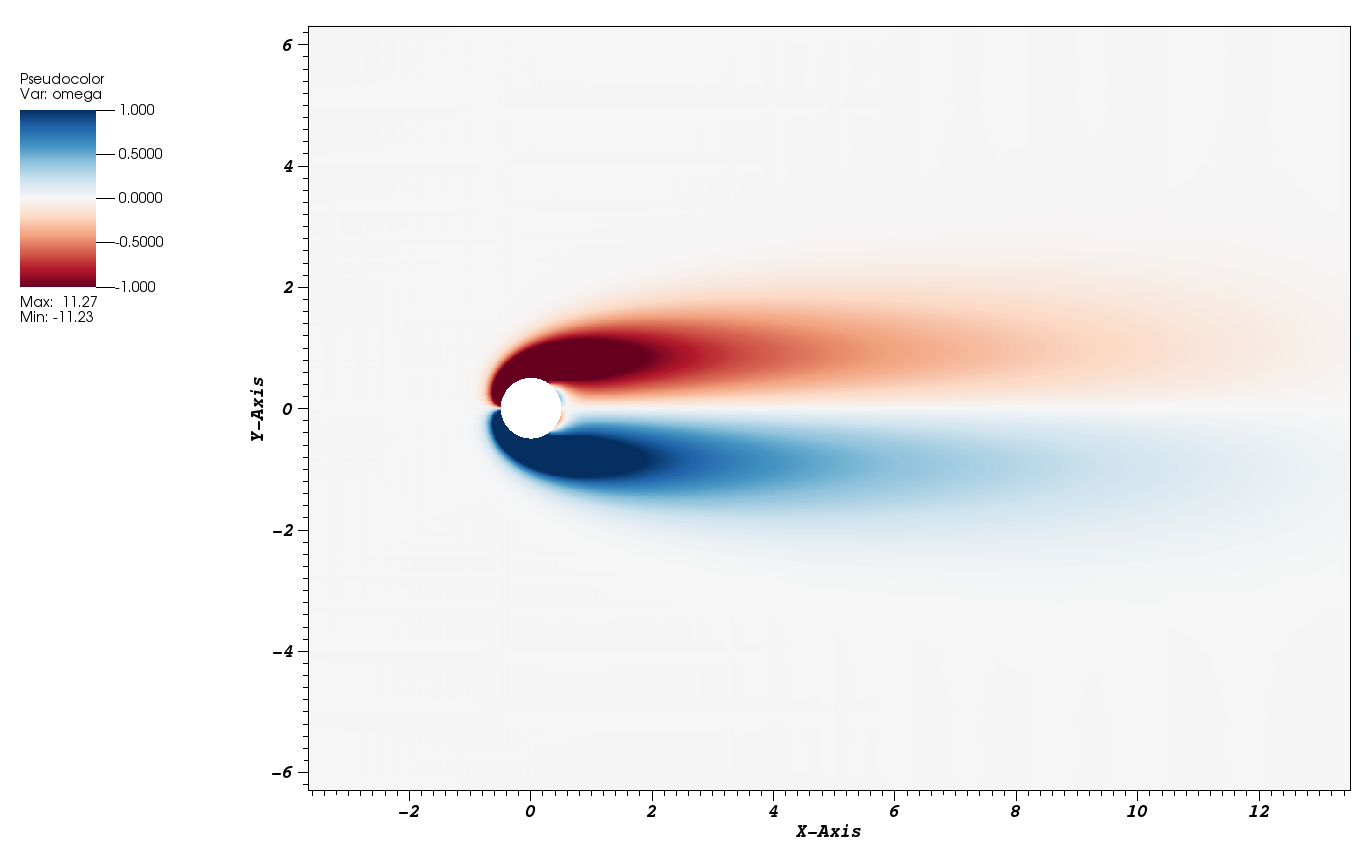
\includegraphics[height=10cm]{Re20DG3CpD60.png}
	\caption{Vorticity for DG3CpD60 for $\text{Re} = 20$}
	\label{fig:vorticity20}
\end{figure}	

	\subsubsection{Simulation at Reynolds Number 40}
	As we did for $\text{Re}=20$, we will now compare our results for the wake separation length and the coefficient of drag to those documented before by others. Once again, we compare our result simulated with DG3CpD60 which now is much more accurate than it was for $\text{Re}=20$. The coefficient of drag is slightly too high but still in very good agreement; the wake separation length is much higher which is caused by the coarse mesh for $x,y \geq 2$. As we expected before, we can confirm the theory that higher Reynolds number cause higher wake separation lengths.
\begin{table}[htp]
	\centering
	\begin{tabular}{|l|l|c|c|c|}
		\hline
		\rule{0pt}{2,3ex}$\text{Re}=40$                              & Source                             & \gls{2d}/\gls{3d} & $W^*$ & $C_D$ \\ \hline
		\rule{0pt}{2,3ex}\multirow{3}{*}{\begin{minipage}{2.8cm}Numerical --\newline Incompressible\end{minipage}} & Dennis et al {[}1970{]}            & \gls{2d}    & $2.35$     & $1.52 $    \\ \cline{2-5} 
		\rule{0pt}{2,3ex}& Forberg {[}1980{]}                 & \gls{2d}    & $2.24$     & $1.50 $   \\ \cline{2-5} 
		\rule{0pt}{2,3ex}& Linnick et al. {[}2005{]}          & \gls{2d}    &$ 2.28$     & $1.54  $   \\ \hline
		\rule{0pt}{2,3ex}\multirow{2}{*}{Experimental}               & Coutanceau et al. {[}1978{]}       & -     & $2.13 $  & -     \\ \cline{2-5} 
		\rule{0pt}{2,3ex}& Tritton {[}1959{]}                 & -     & -     & $1.59 $    \\ \hline
		\rule{0pt}{2,3ex}\multirow{3}{*}{\begin{minipage}{2.8cm}Numerical --\newline Compressible\end{minipage}}     & Brehm et al. {[}2015{]} (Ma = 0.1) & \gls{3d}    & $2.26$     & $1.51 $    \\ \cline{2-5} 
		\rule{0pt}{2,3ex}& Ayers {[}2015{]}                   & \gls{2d}    & $2.250 $    & $1.605$     \\ \cline{2-5} 
		\rule{0pt}{2,3ex}& \textbf{Present Results:}                   & \gls{2d}    & $2.70$     & $1.61 $    \\ \hline
	\end{tabular}	
	\caption{Comparison of Results for $W^*$ and $C_D$, taken from \cite{ayers}, modified}
	\label{table40}
\end{table}
In \cref{C_D40,W40}, you can see the results of every simulation. As we did for $\text{Re}=20$, we did not simulate DG3CpD80 as it would have taken too long. Unfortunately, we did not get a stable calculation for DG3CpD40 until we reduced the time step by ninety-five per cent. This resulted into a tremendous runtime which made the simulation impossible. \\\indent
\begin{table}[htp]
	\centering
	\def\arraystretch{1.5}
%	\begin{minipage}[b]{0.3\textwidth}	
		\begin{tabular}{|c|c|c|c|c|}
			\hline
			\multicolumn{2}{|c|}{\multirow{2}{*}{$C_D$}} & \multicolumn{3}{c|}{CpD} \\ \cline{3-5} 
			\multicolumn{2}{|c|}{}                       & 40     & 60    & 80    \\ \hline
			\multirow{3}{*}{DG}            & 1           &   $1.3729380901298$     &     $1.46072184744588$  &     $1.48507770769867$   \\ \cline{2-5} 
			& 2           &     $1.60025832690217$   &   $1.59617303474342$    &     $1.6161797186352$   \\ \cline{2-5} 
			& 3           &      -  &     $1.60757505790039$  &     -   \\ \hline
		\end{tabular}
		\caption[$C_D$ Values for each simulation]{$C_D$ Values for Each Simulation ($\text{Re} = 40$)}	
		\label{C_D40}
	\end{table}
	\begin{table}[htp]
	\centering
	\def\arraystretch{1.5}
%	\end{minipage}
%	\centering
%	\quad
%	\begin{minipage}[b]{0.3\textwidth}	
		\begin{tabular}{|c|c|c|c|c|}
			\hline
			\multicolumn{2}{|c|}{\multirow{2}{*}{$W^*$}} & \multicolumn{3}{c|}{CpD} \\ \cline{3-5} 
			\multicolumn{2}{|c|}{}                       & 40     & 60    & 80    \\ \hline
			\multirow{3}{*}{DG}            & 1           &    $2.841796875$    &    $2.837890625$   &    $2.736328125$    \\ \cline{2-5} 
			& 2           &     $2.615234375$   &    $2.681640625$   &     $2.681640625$   \\ \cline{2-5} 
			& 3           &     -   &    $2.701171875$   &    -    \\ \hline
		\end{tabular}
		\caption{Wake Separation Lengths for Each Simulation ($\text{Re} = 40$)}	
		\label{W40}
%	\end{minipage} 
\end{table}
In \cref{fig:C_D40} you can see the graphical presentation of \cref{C_D40}; here it is very clear that higher order calculations provide even for coarse meshes very accurate solutions. \\\indent
	\begin{figure}[htp]	
		\centering
		\begin{tikzpicture}
		\begin{semilogxaxis}[xlabel ={Cells per Direction}, ylabel ={$C_D$},  grid =major, legend entries ={$P=1$, $P = 2$, $P=3$}, unbounded coords=jump, legend style = {cells = {anchor=east}, legend pos=outer north east,}, scaled x ticks = false, scaled y ticks = false, xmin = 40, xmax = 80]
		\addplot table[ x = ms, y =dg1] {data/re40.dat};
		\addlegendentry{$P=1$}
		\addplot table[ x = ms, y =dg2] {data/re40.dat};
		\addlegendentry{$P=2$}
		\addplot table[ x = ms, y =dg3] {data/re40.dat};
		\addlegendentry{$P=3$}
%		\addplot[mark=none, red] coordinates {(32, 1.6) (128, 1.6)};
%		\addlegendentry{Constant Value}
		\end{semilogxaxis}	
		\end{tikzpicture}
		\caption{Graphical Presentation of Table \ref{C_D40} for $\text{Re} = 40$}
		\label{fig:C_D40}	
	\end{figure}
\begin{figure}[htp]	
	\centering
	\begin{tikzpicture}
	\begin{semilogyaxis}[xlabel ={Time}, ylabel ={$C_D$},  grid =major, unbounded coords=jump, legend style = {cells = {anchor=east}, legend pos=outer north east}, scaled x ticks = false, scaled y ticks = false, xmin = 0, xmax = 14]
	\addplot[brown] table[x = t, y =C_D, mark=none] {data/re40dg1cpd40.dat};
	\addlegendentry{DG1CpD40}
	\addplot[red] table[ x = t, y =C_D, mark=none] {data/re40dg2cpd60.dat};
	\addlegendentry{DG2CpD60}
	\addplot[blue] table[ x = t, y =C_D, mark=none] {data/re40dg3cpd60.dat};
	\addlegendentry{DG3CpD60}
	\addplot[black] table[ x = t, y =C_D, mark=none] {data/re40dg2cpd80.dat};
	\addlegendentry{DG2CpD80}
	%		\addplot[mark=none, red] coordinates {(32, 1.6) (128, 1.6)};
	%		\addlegendentry{Constant Value}
	\end{semilogyaxis}	
	\end{tikzpicture}
	\caption{Coefficient of Drag over Time ($\text{Re} = 40$)}
	\label{fig:C_Dt40}	
\end{figure}
As you can see in \cref{fig:C_Dt40}, the behaviour of the coefficient of drag over the physical time is very similar for the simulations plotted. They are more in agreement with each other than they were for $\text{Re = 20}$. In \cref{fig:vorticity40}, you can see the vorticity for DG3CpD60; there we remark that the wake is much longer than it was for $\text{Re}=20$.
\begin{figure}[htp]
	\centering
	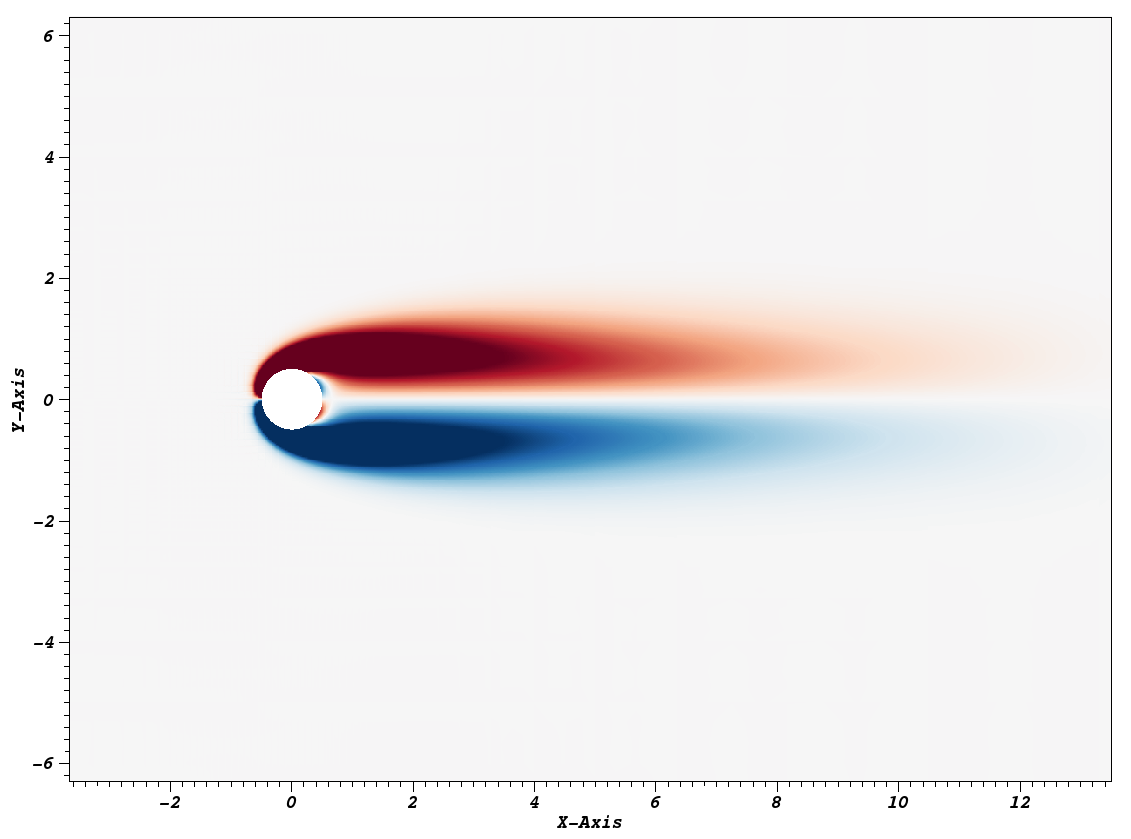
\includegraphics[height=10cm]{Re40DG3CpD60.png}
	\caption{Vorticity for DG3CpD60 for $\text{Re} = 40$}
	\label{fig:vorticity40}
\end{figure}
	\subsection{Unsteady Simulations ($\text{Re}> 40-50$)}
	After having examined the steady simulations which were very accurate for the coefficient of drag, we will now turn to the unsteady ones with $\text{Re}=100$ and $\text{Re}=200$.
	In order to compare the unsteady simulations we need the Strouhal number
	\begin{align}
		\text{St} = \dfrac{f  L_\infty}{V_\infty}.
	\end{align}
	As our initial and boundary conditions give $V_\infty = L_\infty = 1$, we can calculate $\text{St} = f$ with $f$ found from examining the oscillation of $C_L$ over time. In order to develop vortex shedding, the flow needs small perturbations that destabilise the flow towards a symmetry breaking state (\textcite{FLM:14223}). In reality those are given by the structure of the cylinder, the influence of the walls or the not completely straight inflow; in our simulations they come from small truncation errors and the computer's round-off errors. 
	In order to accelerate the process until the wake begins to oscillate, one could also start the flow with a vortex that induces a high perturbation much earlier. For it did not take long until the wake began to oscillate it was not needed in our simulations.
	\subsubsection{Simulation at Reynolds Number 100}
\begin{table}[htp]
	\centering
	\begin{tabular}{|l|p{4cm}|c|c|c|c|}
		\hline
		\rule{0pt}{2,3ex}$\text{Re}=100$                              & Source                             & \gls{2d}/\gls{3d} & $St$ & $C_D$ & $C_L$\\ \hline
		\rule{0pt}{2,3ex}\multirow{7}{*}{\begin{minipage}{2.8cm}Numerical --\newline Incompressible\end{minipage}} & Gresho et al. {[}1984{]}            & \gls{2d}    & $0.18$     & $1.76$ & -   \\ \cline{2-6} 
		\rule{0pt}{2,3ex}& Linnick et al. {[}2005{]} \newline ($\lambda = 0.056$)                 & \gls{2d}    & $0.169$     & $1.38 \pm 0.010$  &  $\pm  0.337 $\\ \cline{2-6} 
		\rule{0pt}{2,3ex}& Linnick et al. {[}2005{]} \newline ($\lambda = 0.023$)                  & \gls{2d}    & $0.1696 $   & $1.34 \pm 0.009$  & $ \pm 0.333 $\\ \cline{2-6} 
		\rule{0pt}{2,3ex}& Persillon et al. {[}1998{]}                 & \gls{2d}    & $0.165  $   &$ 1.253 $ & -  \\ \cline{2-6} 
		\rule{0pt}{2,3ex}& Saiki et al. {[}1996{]}                 & \gls{2d}    &$ 0.171  $   & $1.26 $ &  - \\ \cline{2-6} 
		\rule{0pt}{2,3ex}& Persillon et al. {[}1998{]}                 & \gls{3d}    & $0.164$     & $1.240 $ & -  \\ \cline{2-6} 
		\rule{0pt}{2,3ex}& Liu et al. {[}1998{]}          & \gls{3d}    &$ 0.165 $    & $1.35 \pm 0.012$  &$ \pm 0.339 $ \\ \hline
		\rule{0pt}{2,3ex}\multirow{2}{*}{Experimental}               & Berger et al. {[}1972{]}       & -     &$ 0.16-0.17 $   & -    & -\\ \cline{2-6} 
		\rule{0pt}{2,3ex}& Clift et al. {[}1978{]}                 & -    & -     &$ 1.24 $ &  - \\ \cline{2-6} 
		\rule{0pt}{2,3ex}& Williamson {[}1996{]}                 & -     &$ 0.164  $  & -   & - \\ \hline
		\rule{0pt}{2,3ex}\multirow{3}{*}{\begin{minipage}{2.8cm}Numerical -- \newline Compressible\end{minipage}}     & Brehm et al. {[}2015{]} \newline (Ma = 0.1) & \gls{3d}    & $0.165$    &$ 1.32 \pm 0.01  $  & $\pm 0.32 $\\ \cline{2-6} 
		\rule{0pt}{2,3ex}& Ayers {[}2015{]}                   & \gls{2d}    &$ 0.167$     & $1.371 \pm 0.011 $ &$ \pm 0.333 $\\ \cline{2-6} 
		\rule{0pt}{2,3ex}& \textbf{Present Results:}                   & \gls{2d}    & d     & 4  &   \\ \hline
	\end{tabular}	
	\caption{Comparison of Results for $St$, $C_D$ and $C_L$, taken from \cite{ayers}, modified}
	\label{table100}
\end{table}


	
		\begin{figure}[htp]	
			\centering
			\begin{tikzpicture}
				\begin{axis}[xlabel ={Time}, ylabel ={$C_L$}]%, grid =major, legend entries ={$P=1$}, unbounded coords=jump, legend style = {cells = {anchor=east}, legend pos=outer north east,}, scaled x ticks = false, xmin = 0, xmax = 120]
				\addplot table[ x = time, y = l, mark=none] {data/ms64dg1re100.dat};
				\end{axis}	
			\end{tikzpicture}
			\caption{Lift coefficient over time for Re = 100}
			\label{osci100}	
		\end{figure}
%		\begin{figure}[htp]	
%			\centering
%			\begin{tikzpicture}
%			\begin{axis}[xlabel ={Time}, ylabel ={$C_L$}, grid =major, legend entries ={$P=1$}, unbounded coords=jump, legend style = {cells = {anchor=east}, legend pos=outer north east,}, scaled x ticks = false]
%			\addplot table[ x = time, y = l, mark = none] {data/re100dg1ms128.dat};
%			\end{axis}	
%			\end{tikzpicture}
%			\caption{Convergence Plot}
%			\label{shijfterror}	
%		\end{figure}
%		\begin{figure}[htp]	
%			\centering
%			\begin{tikzpicture}
%			\begin{axis}[xlabel ={Time}, ylabel ={$C_L$},  grid =major, legend entries ={$P=1$}, unbounded coords=jump, legend style = {cells = {anchor=east}, legend pos=outer north east,}, scaled x ticks = false, scaled y ticks = false, xmin = 300, xmax = 350]
%			\addplot table[ x =time, y =l, mark=none] {data/re100dg1ms128.dat};
%			\end{axis}	
%			\end{tikzpicture}
%			\caption{Convergence Plot}
%			\label{shijfterror}	
%		\end{figure}
	\subsubsection{Simulation at Reynolds Number 200}
\begin{table}[htp]
	\centering
	\begin{tabular}{|l|p{4cm}|c|c|c|c|}
		\hline
		\rule{0pt}{2,3ex}$\text{Re}=200$                              & Source                             & \gls{2d}/\gls{3d} & $St$ & $C_D$ & $C_L$\\ \hline
		\rule{0pt}{2,3ex}\multirow{9}{*}{\begin{minipage}{2.8cm}Numerical --\newline Incompressible\end{minipage}} & Belov et al. {[}1995{]}            & \gls{2d}    & $0.193$     & $1.19 \pm 0.042$ & $\pm 0.64$   \\ \cline{2-6} 
		\rule{0pt}{2,3ex} & Gresho et al. {[}1984{]}            & \gls{2d}    & $0.21$     & $1.76$ & -   \\ \cline{2-6} 
		\rule{0pt}{2,3ex}& Linnick et al. {[}2005{]} \newline ($\lambda = 0.056$)                 & \gls{2d}    & $0.199$     & $1.37 \pm 0.046$  &  $\pm  0.70$\\ \cline{2-6} 
		\rule{0pt}{2,3ex}& Linnick et al. {[}2005{]} \newline ($\lambda = 0.023$)                  & \gls{2d}    & $0.197 $   & $1.34 \pm 0.044$  & $ \pm 0.69$\\ \cline{2-6} 
		\rule{0pt}{2,3ex}& Miyake et al. {[}1992{]}                 & \gls{2d}    & $0.196$   &$1.34 \pm 0.043 $ & $\pm 0.67$  \\ \cline{2-6} 
		\rule{0pt}{2,3ex}& Persillon et al. {[}1998{]}                 & \gls{2d}    & $0.198  $   &$ 1.321 $ & -  \\ \cline{2-6} 
		\rule{0pt}{2,3ex}& Saiki et al. {[}1996{]}                 & \gls{2d}    &$ 0.197  $   & $1.18 $ &  - \\ \cline{2-6} 
		\rule{0pt}{2,3ex}& Persillon et al. {[}1998{]}                 & \gls{3d}    & $0.181$     & $1.306 $ & -  \\ \cline{2-6} 
		\rule{0pt}{2,3ex}& Liu et al. {[}1998{]}          & \gls{3d}    &$ 0.192 $    & $1.31 \pm 0.049$  &$ \pm 0.69 $ \\ \hline
		\rule{0pt}{2,3ex}\multirow{2}{*}{Experimental}               & Berger et al. {[}1972{]}       & -     &$ 0.18-0.19 $   & -    & -\\ \cline{2-6} 
		\rule{0pt}{2,3ex}& Clift et al. {[}1978{]}                 & -    & -     &$ 1.16 $ &  - \\ \cline{2-6} 
		\rule{0pt}{2,3ex}& Williamson {[}1996{]}                 & -     &$ 0.181  $  & -   & - \\ \hline
		\rule{0pt}{2,3ex}\multirow{3}{*}{\begin{minipage}{2.8cm}Numerical --\newline Compressible\end{minipage} }    & Brehm et al. {[}2015{]} \newline (Ma = 0.1) & \gls{3d}    & $0.192$    &$ 1.3 \pm 0.04  $  & $\pm 0.66 $\\ \cline{2-6} 
		\rule{0pt}{2,3ex}& Ayers {[}2015{]}                   & \gls{2d}    &$ 0.201$     & $1.371 \pm 0.011 $ &$ \pm 0.70 $\\ \cline{2-6} 
		\rule{0pt}{2,3ex}& \textbf{Present Results:}                   & \gls{2d}    & d     & 4  &   \\ \hline
	\end{tabular}	
	\caption{Comparison of Results for $St$, $C_D$ and $C_L$, taken from \cite{ayers}, modified}
	\label{table200}
\end{table}
	
			\begin{figure}[htp]	
				\centering
				\begin{tikzpicture}
				\begin{axis}[xlabel ={Time}, ylabel ={$C_L$}, grid =major, legend entries ={$P=1$}, unbounded coords=jump, legend style = {cells = {anchor=east}, legend pos=outer north east,}, scaled x ticks = false]
				\addplot table[ x =time, y =l, mark=none] {data/re200dg1.dat};
				\end{axis}	
				\end{tikzpicture}
				\caption{Lift coefficient over time for Re=200}
				\label{osci200}	
			\end{figure}